\documentclass[12pt,a4paper,notitlepage]{article}
\usepackage[T1]{fontenc}
\usepackage[top=3cm, bottom=2.5cm, left=3cm, right=3cm]{geometry}
\usepackage[OT4]{polski}
\usepackage[section]{placeins}
\usepackage[utf8]{inputenc} 
\usepackage{longtable}
\linespread{1.3}
\usepackage{color}
\definecolor{bluekeywords}{rgb}{0.13,0.13,1}
\definecolor{greencomments}{rgb}{0,0.5,0}
\definecolor{redstrings}{rgb}{0.9,0,0}
\usepackage{listings}
\lstset{language=Java,
showspaces=false,
showtabs=false,
breaklines=true,
showstringspaces=false,
breakatwhitespace=true,
escapeinside={(*@}{@*)},
commentstyle=\color{greencomments},
keywordstyle=\color{bluekeywords}\bfseries,
stringstyle=\color{redstrings},
basicstyle=\ttfamily}
\usepackage{float}
\usepackage{graphicx}

\renewcommand\lstlistlistingname{Spis listingów}

\begin{document}
\makeatletter
\newcommand{\linia}{\rule{\linewidth}{0.4mm}}
\renewcommand{\maketitle}{\begin{titlepage}
    \vspace*{1cm}
    \begin{center}\small
    Politechnika Wrocławska\\
    Wydział Elektroniki
    \end{center}
    \vspace{3cm}
    \noindent\linia
    \begin{center}
      \LARGE \textsc{\@title}\\
      \large System do ankietowania na stronie WWW
         \end{center}
     \linia
    \vspace{0.5cm}
    \begin{flushright}
    \begin{minipage}{6cm}
    \textit{\small Autor:}\\
    \normalsize \textsc{\@author} \par
    \end{minipage}
    \vspace{5cm}\\
     {\small Promotor:}\\
         dr inż. Roman Ptak
     \end{flushright}
    \vspace*{\stretch{6}}
    \begin{center}
    \@date
    \end{center}
  \end{titlepage}%
}
\makeatother
\author{Marcin Wincek 196099 }
\title{Projekt inżynierski}
\date{10.12.2014 r.}

\maketitle

\setcounter{page}{2}
\tableofcontents



\section{Wstęp}
\subsection{Wprowadzenie}
Wiele dziedzin przemysłu wykorzystuje badania opinii publicznej za pomocą ankietcelu podniesienia jakości swoich usług. Ankietowanie nie musi dotyczyć tylko przemysłu, może dotyczyć wielu innych dziedzin życia. Współczesne technologie informatyczne pozwalają zautomatyzować proces ankietowania przez zbieranie odpowiedzi do ankiet w~bazie danych oraz automatyczną analizę danych. Pozwala to na znaczne usprawnienie tego procesu, a~co za tym idzie - zyski finansowe, mniej wysiłku wymaganego od ankietującego, czy też większy komfort dla ankietowanego. 

\subsection{Cel i~zakres projektu}
Celem projektu jest stworzenie aplikacji internetowej pełniącej rolę systemu do ankietowania. Aplikacja będzie dostępna dla użytkowników w~formie strony internetowej. System powinien spełniać podstawowe wymagania, tj.:
\begin{itemize}
\item tworzenie ankiet,
\item zbieranie odpowiedzi od respondentów,
\item analiza zebranych odpowiedzi.
\end{itemize}
\par Aplikacja dostarczy użytkownikom możliwości tworzenia i~edycji ankiet oraz analizy ich wyników. System będzie generował dla każdej ankiety osobną stronę dla respondentów, a~hiperłącze do tej strony będzie udostępniał dla użytkownika tworzącego ankietę. Projekt nie zakłada automatycznego rozsyłania linka do respondentów.
\par Na stronie udostępnianej respondentom wyświetlane będą pytania ankiety. Respondenci będą mieli możliwość udzielenia odpowiedzi na wszystkie pytania oraz wysłanie ich do systemu. Projekt zakłada, że każdy respondent będzie mógł wypełnić ankietę tylko jeden raz.

\newpage
\section{Analiza wymagań systemowych}

\subsection{Przypadki użycia aplikacji}
W systemie wyszczególniono dwa typy użytowników: 
\begin{itemize}
\item użytkownik tworzący ankietę,
\item respondent.
\end{itemize}
Dla każdego z~typów określono typowe przypadki użycia aplikacji.
\subsubsection{Autor ankiety}
Rysunek 1. przedstawia przypadki użycia aplikacji przez autora ankiety.
\begin{figure}[H]
\begin{center}
\scalebox{0.75}{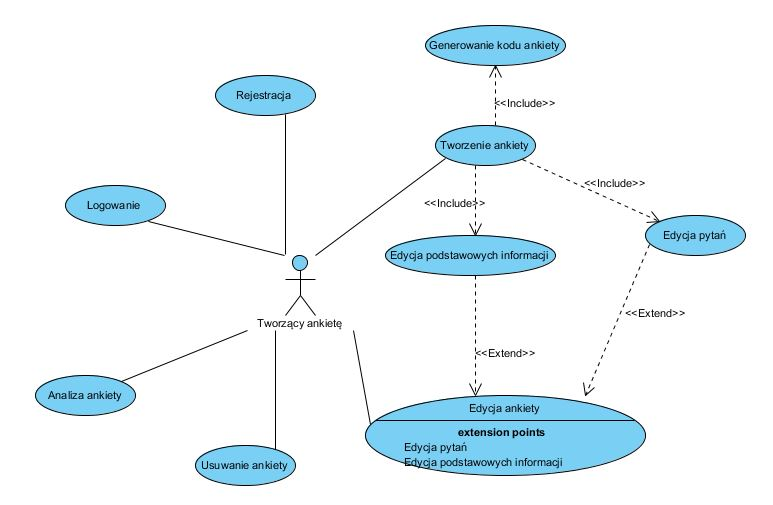
\includegraphics{obrazy/useCaseAuthor}}
\caption{Diagram przypadków użycia dla tworzącego ankietę}
\end{center}
\end{figure}
Użytkownik chcąc skorzystać z~systemu musi wcześniej zalogować się do niego, a~jeśli nie posiada jeszcze własnego konta, musi takowe stworzyć. Po zalogowaniu się do serwisu może korzystać ze wszystkich funkcjonalności. Najbardziej rozbudowanymi z~nich jest tworzenie nowej ankiety oraz edycja już stworzonych. Użytkownik ma również możliwość usunięcia swojej ankiety z~systemu. 

\subsubsection{Respondent}
Rysunek 2. przedstawia przypadki użycia aplikacji przez respondenta.
\begin{figure}[H]
\begin{center}
\scalebox{0.75}{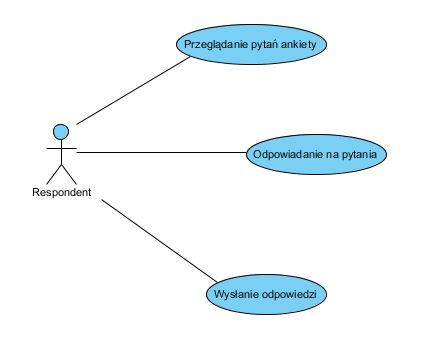
\includegraphics{obrazy/useCaseRespondent}}
\caption{Diagram przypadków użycia dla respondenta}
\end{center}
\end{figure}

Użytkownik udzielający odpowiedzi w~ankiecie ma mniej możliwości w~systemie. Jego zadaniem jest udzielenie odpowiedzi na pytania i~wysłanie tych odpowiedzi na serwer.

\subsection{Wymagania funkcjonalne}
Analiza przypadków użycia pozwala wyselekcjonować funkcjonalności, jakie system powinien oferować użytkownikom. Wymagania funkcjonalne postawione przed systemem zostały przedstawione w~formie tabeli. Kolejność zawartych w~niej funkcjonalności jest chronologicznym odzwierciedleniem kolejności ich implementacji. O~krytyczności danej funkcjonalności decyduje jej niezbędność w~systemie. W~przedstawionej tabeli charakterystyka krytyczności została opisana w~skali czterostopniowej: wysoka, średnia, niska oraz dodatkowa. Wysokiej krytyczności są funkcjonalności będące absolutnym filarem działania systemu, zaś elementy dodatkowe nie wnoszą niczego do funkcjonalności, lecz pozwalają na wykonanie tych samych czynności w~inny, bardziej komfortowy sposób. Tabela 1. przedstawia dokładną analizę wymagań funkcjonalnych.

\begin{center}
\begin{table}
\caption{Spis wymagań funkcjonalnych}
  \begin{tabular}{| c| c|}%left i~center wyrownanie

    \hline
    Opis & Krytyczność \\ \hline \hline
   Rejestracja kont użytkowników w~systemie	&	Wysoka	\\ \hline
   
   
Logowanie na konta użytkowników	&	Wysoka	\\ \hline


Zmiana danych osobowych przez użytkowników & Dodatkowa	\\ \hline


Tworzenie ankiety 	&	Wysoka	\\ \hline

Usuwanie ankiety & Średnia \\ \hline


Edycja pytań 	&	Wysoka	\\ \hline

Edycja podstawowych informacji ankiety &	Średnia 	\\ \hline


Generowanie kodu ankiety	&	Wysoka	\\ \hline


Możliwość oddawania głosów w~ankiecie 	&	Wysoka	\\ \hline

Generowanie wykresów z~wyników ankiety	&	Wysoka	\\ \hline

Eksportowanie wyników ankiety do zewnętrznych plików	&	Dodatkowa	\\ \hline

Pobieranie wyników ankiety w~czasie rzeczywistym & Niska \\ \hline

Automatyczne rozsyłanie linków do ankiety na wskazane adresy email & Dodatkowa \\ \hline


    \hline
  \end{tabular}
\end{table}
\end{center}


\subsection{Wymagania niefunkcjonalne}
Aplikacja została przetestowana i~działała poprawnie na następujących przeglądarkach internetowych:
\begin{itemize}
\item Google Chrome 37,
\item Mozilla Firefox 31,
\item Opera 22,
\item Internet Explorer 9.
\end{itemize}
Działanie aplikacji na niższych wersjach tych przeglądarek może (ale nie musi) być niezgodne z~wymaganiami. Autor aplikacji nie gwarantuje poprawnego działania na przeglądarkach nie wymienionych powyżej. Wyjątkiem tutaj jest Internet Explorer, który od wersji 8~w dół nie jest wspierany.
\par Aplikacja powinna zapewniać bezpieczeństwo przetwarzanych danych, a~szczególnie danych osobowych. W~tym celu należy zabezpieczyć połączenie między klientem a~serwerem za pomocą odpowiedniego protokołu (SSL).
\par Przeglądarka internetowa, za pomocą której użytkownik korzysta z~aplikacji musi mieć włączoną obsługę JavaScript.
\par Aplikacja serwerowa powinna dać się uruchomić na maszynie z~systemem operacyjnym Windows lub Linux (dystrybucje Ubuntu lub Debian).

\subsection{Przegląd innych rozwiązań}
W Internecie można znaleźć wiele rozwiązań podobnych do tworzonego systemu. Wiele z~nich, oprócz podstawowych funkcjonalności, zapewnia również ciekawe dodatki, takie jak automatyczne powiadomienia dla autora o~nowych odpowiedziach, wiele dodatkowych typów pytań, możliwość skorzystania z~predefiniowanych pytań itp. Niestety, takie dodatkowe funkcjonalności są często dostępne po zapłaceniu dodatkowych opłat. Poniżej wymienione zostały przykłady aplikacji do ankietowania.

\subsubsection{Google Docs}
Google Docs to prawdopodobnie najpopularniejsze narzędzie wykorzystywane do przeprowadzania ankiet. Jest to rozwiązanie w~pełni darmowe, do korzystania potrzebne jest tylko konto w~serwisie Gmail. System pozwala w~łatwy sposób stworzyć ankietę i~udostępnić ja dla respondentów. Serwis Google Docs daje możliwość stworzenia ankiety składającej się z~wielu pytań, istnieje również wiele możliwych typów pytań (dokładnie 9). Tworzenie przyładowej ankiety przedstawione zostało na Rysunku 3.
\par Sporą wadą tej aplikacji jest fakt, że po przeprowadzeniu ankiety wyniki dostarczane są w~postaci surowego arkusza kalkulacyjnego. Dalsze kroki analizy ankiety, takie jak wykresy itp., trzeba przeprowadzić samemu.
\paragraph{Zalety}
\begin{itemize}
\item Rozwiązanie darmowe
\item Łatwość stworzenia ankiety
\item Wiele typów pytań
\end{itemize}

\paragraph{Wady}
\begin{itemize}
\item Słaba analiza wyników ankiety.
\end{itemize}

\begin{figure}[H]
\begin{center}
\scalebox{0.67}{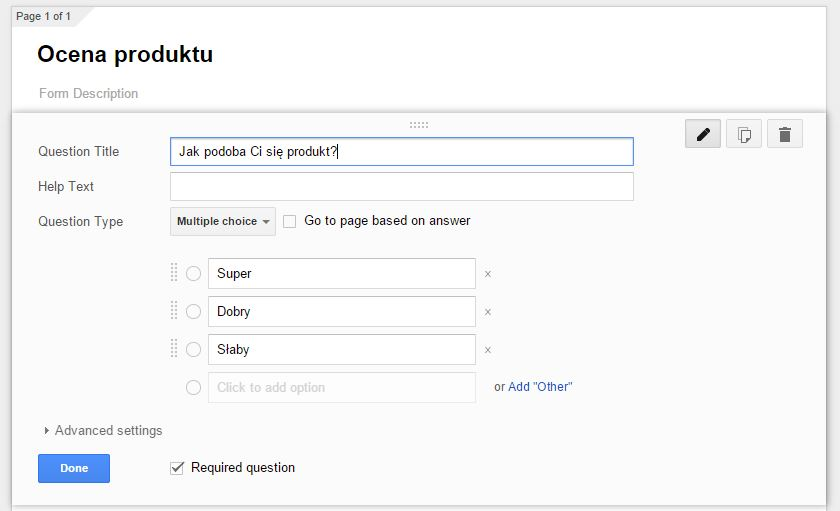
\includegraphics{obrazy/googleDocs}}
\caption{Okno tworzenia ankiety w~Google Docs}
\end{center}
\end{figure}

\subsubsection{Ankietka.pl}
Ankietka.pl jest serwisem polskim, prawdopodobnie najpopularniejszym w~naszym kraju. W~przeciwieństwie do Google Docs jest tylko częściowo darmowy. W~darmowej wersji serwisu napotkać można znaczące ograniczenia, np. limit respondentów per ankieta (30). Dodatkowo korzystając z~darmowej wersji nasza ankieta będzie umieszczona w~publicznie dostępnej Bazie ankiet, co może być niepożądane.
\par Decydując się jednak na płatną wersję (najtańsze rozwiązanie - 39 zł/msc) mamy do dyspozcji wiele przydatnych funkcji, np. eksport wyników do zewnętrznych plików, ukrycie ankiety w~Bazie ankiet, brak reklam w~serwisie.
\par Rysunek 4. przedstawia przykładową analizę odpowiedzi do ankiety.

\paragraph{Zalety}
\begin{itemize}
\item Wiele typów pytań
\item Rozwinięta analiza odpowiedzi (wykresy)
\item Możliwość eksportu do pliku
\end{itemize}

\paragraph{Wady}
\begin{itemize}
\item Ograniczenia w~darmowej wersji
\item Zapisywanie ankiety do bazy ankiet
\item Pełna funkcjonalność po zapłaceniu (min. 39 zł/msc)
\end{itemize}

\begin{figure}[H]
\begin{center}
\scalebox{0.67}{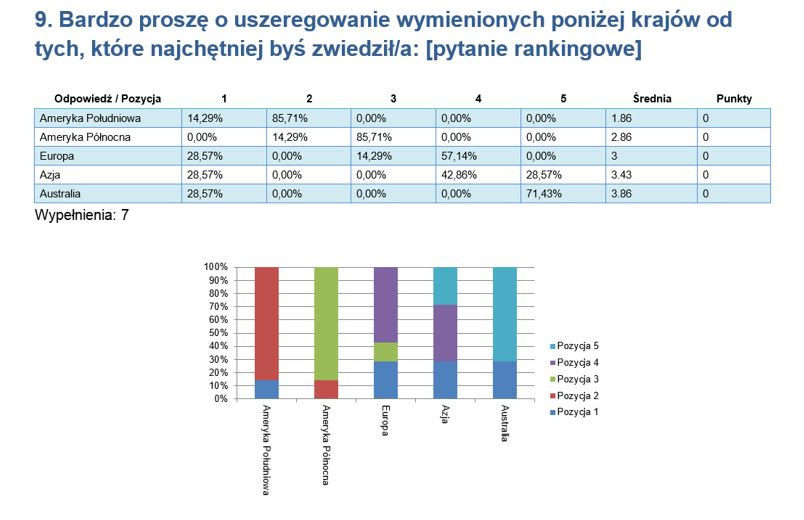
\includegraphics{obrazy/ankietkapl}}
\caption{Przykładowe okno analizy wyników ankiety w~serwisie Ankietka.pl}
\end{center}
\end{figure}

\subsubsection{SurveyMonkey.com}
Jako ostatni omówiony zostanie serwis SurveyMonkey.com. W~porównaniu z~wcześniej przedstawionymi rozwiązaniami, SurveyMonkey.com jest najbardziej rozbudowanym, profesjonalnym narzędziem, powszechnie używanym przez wiele światowych firm (Facebook, Samsung, Virgin). Jak można się spodziewać, za wysoką jakość trzeba zapłacić. Podobnie jak na stronie Ankietka.pl istnieje darmowa wersja serwisu, jednak ograniczenia są bardzo duże: limit pytań w~ankiecie - 10, limit odpowiedzi - 100. W~płatnej wersji (najtańsza wersja - 75 zł/msc) otrzymujemy wiele użytecznych funkcji, opisanych niżej. Dokładna oferta serwisu została przedstawiona na Rysunku 5.

\paragraph{Zalety}
\begin{itemize}
\item Kompleksowe, profesjonalne narzędzie
\item Bezpieczeństwo rozwiązania (SSL)
\item Konfigurowalny wygląd ankiety
\item Analiza tekstu dla otwartych pytań
\end{itemize}

\paragraph{Wady}
\begin{itemize}
\item Ograniczenia w~bezpłatnej wersji
\item Większość funkcjonalności dostępna w~płatnej części serwisu (minimum 75 zł/msc)
\end{itemize}

\begin{figure}[H]
\begin{center}
\scalebox{0.67}{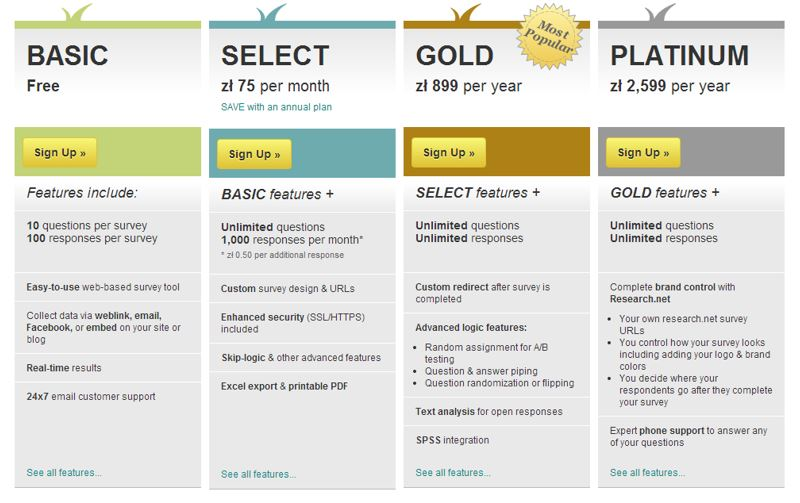
\includegraphics{obrazy/surveyMonkey}}
\caption{Oferta serwisu SurveyMonkey.com}
\end{center}
\end{figure}

\newpage

\section{Architektura systemu}
\subsection{Organizacja aplikacji}
Aplikację tworzą trzy oddzielne części:
\begin{itemize}
\item serwer HTTP (node.js),
\item baza danych (mongoDB),
\item warstwa kliencka (AngularJS).
\end{itemize}
Tego typu architektura określana jest mianem MEAN (\textbf{M}ongoDB, \textbf{E}xpress.js, \newline \textbf{A}ngular.js, \textbf{N}ode.js).
Serwer HTTP udostępnia REST'owe API, będące podstawowym kanałem komunikacji między klientem a~serwerem. API zostało dokładniej opisane w~punkcie 4.3.
\par W~przeciwieństwie do tradycyjnego podejścia do tworzenia aplikacji internetowych, w~projekcie zastosowano koncepcję Single Page Application. Polega ona na tym, że przy przechodzeniu między poszczególnymi widokami nie jest wymagane pobranie całej zawartości strony (HTML + arkusze stylów + skrypty), ale jedynie części widoku. Część kliencka aplikacji (Angular) wykonuje zapytanie typu AJAX do serwera i~w odpowiedzi otrzymuje fragment strony HTML, który to fragment zostaje umieszczony w~zdefiniowanym przez programistę miejscu. Wszelkie dane dynamiczne (np. dane o~odpowiedziach do ankiety) są pobierane z~serwera w~ten sam sposób.
\par Dane wykorzystywane w~aplikacji przesyłane są pomiędzy poszczególnymi jej częściami w~formacie dokumentów JSON.
\par Rysunek 6. przedstawia architekturę projektowanego systemu.

\begin{figure}[H]
\begin{center}
\scalebox{0.67}{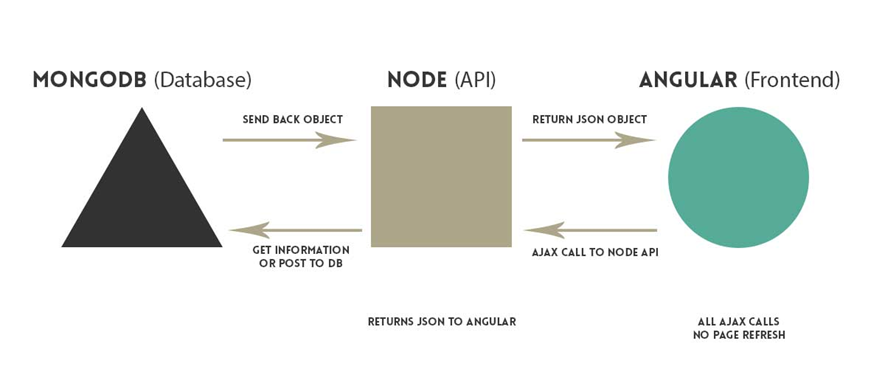
\includegraphics{obrazy/architektura}}
\caption{Architektura aplikacji}
\end{center}
\end{figure}

\par Funkcję persystencji pełni w~aplikacji baza danych MongoDB. Jest to nierelacyjna baza danych, w~której dane są przechowywane w~postaci dokumentów JSON, co ujednolica strukturę danych w~całym projekcie. Więcej informacji o~MongoDB znajduje się w~punkcie 4.1.2.

\par Schodząc na nieco niższy poziom architektury, trzeba opisać strukturę serwera HTTP. Node.js sam w~sobie nie jest widoczny publicznie na porcie 80. W~rzeczywistości wykorzystany został serwer Nginx jako reverse proxy: wszystkie zapytania na port 80 kieruje najpierw na port 443, gdzie dokładane są zabezpieczenia, a~następnie na port 7070, na którym pracuje serwer Node.js.
\par Rysunek 7. przedstawia architekturę systemu wzbogaconą o serwer Nginx.

\begin{figure}[H]
\begin{center}
\scalebox{0.8}{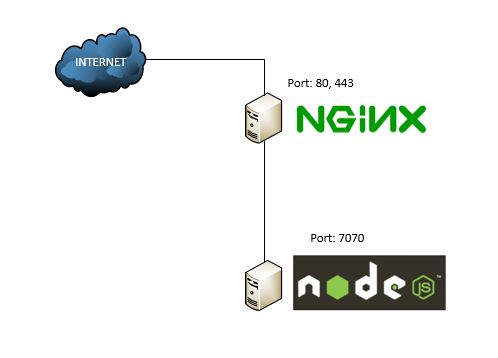
\includegraphics{obrazy/nginx}}
\caption{Zastosowanie Nginx jako reverse proxy}
\end{center}
\end{figure}

\subsection{Struktura bazy danych}
Baza MongoDB jest bazą nierelacyjną, która pozwala na zagnieżdżanie obiektów. Jest to bardzo wygodne, ponieważ użytkownik ma możliwość przechowywania powiązanych ze sobą danych w~jednej kolekcji, co przyspiesza proces wydobywania danych z~bazy - nie ma konieczności tworzenia skomplikowanych często JOIN'ów. Struktura bazy danych przedstawiona została na Rysunku 8.

\begin{figure}[H]
\begin{center}
\scalebox{0.8}{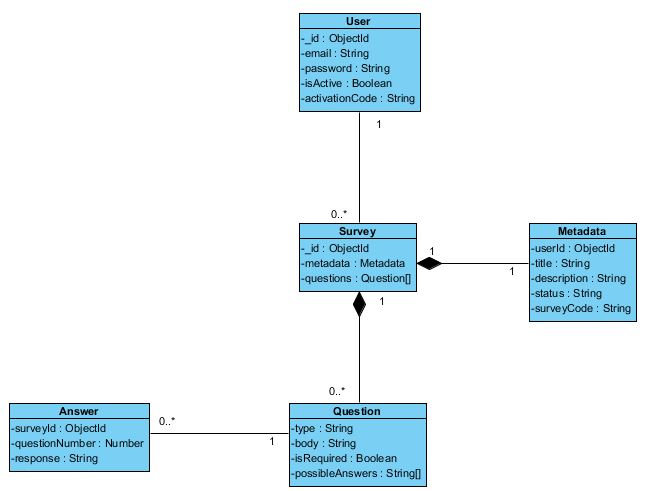
\includegraphics{obrazy/db}}
\caption{Struktura bazy danych}
\end{center}
\end{figure}

\newpage
\section{Implementacja}
\subsection{Wykorzystane technologie}
\subsubsection{Node.js}
Platforma  Node.js jest staje się coraz bardziej popularnym narzędziem do tworzenia aplikacji serwerowych. W~przeciwieństwie do tradycyjnego podejścia (np. Apache), w~Node.js programista sam tworzy serwer HTTP. Wbrew pozorom, stworzenie takiego serwera zajmuje jedną linię kodu.
\par Node.js to biblioteka umożliwiająca wykonywanie skryptów JavaScript dzięki użyciu silnika V8 firmy Google, na której oparty został Google Chrome. Jest rozwiązaniem multiplatformowym, opartym na architekturze sterowanej zdarzeniami. Node.js operuje na jednym wątku, jednak dzięki zastosowaniu nieblokującej obsługi wejścia/wyjścia, pozwala na obsługę dziesiątek tysięcy równoległych połączeń do serwera. Takie asynchroniczne podejście wymaga, aby każda operacja wykorzystująca strumień we/wy używała funkcji zwrotnej (ang. \textit{callback}), która wykonuje się po otrzymaniu danych.
\par Listing 1. pokazuje sposób sposób, w jaki w Node.js obsługuje się operacje asynchroniczne. Jako drugi parametr funkcji przekazywana jest funkcja zwrotna (ang. \texttt{callback}), która zostaje wywołana kiedy przychodzi odpowiedź funkcji \texttt{getSurveyById}.
\begin{lstlisting}[caption=Przykład użycia funkcji zwrotnej w~pobraniu danych z~bazy danych. ]
Surveys.getSurveyById($stateParams.surveyId, function(survey) {
      /**
       * zrob cos
       */
    });
\end{lstlisting}
\par Działanie Node.js opiera się na tzw. pętli zdarzeń. Wszystkie zdarzenia zachodzące podczas działania programu obsługiwane są w~tej pętli w~kolejności, w~jakiej się w~niej znajdą. Takie podejście nie blokuje działania programu, więc mimo faktu, że Node.js działa na jednym wątku, możliwe wysłanie odpowiedzi do wielu klientów jednocześnie. Rysunek 9. pokazuje schemat działania pętli zdarzeń Node.js.

\begin{figure}[H]
\begin{center}
\scalebox{0.8}{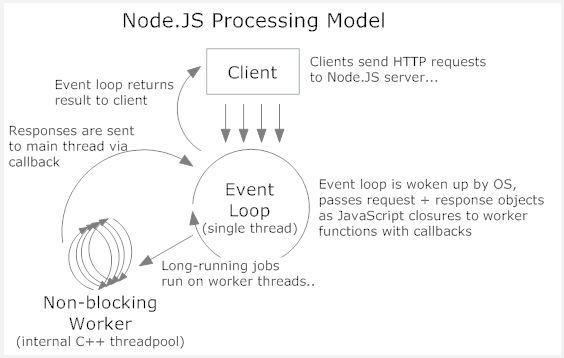
\includegraphics{obrazy/petla}}
\caption{Schemat działania pętli zdarzeń w~Node.js}
\end{center}
\end{figure}

\subsubsection{MongoDB}
MongoDB to nierelacyjny system zarządzania bazą danych napisany w~języku C++. Charakteryzuje się dużą skalowalnością, wydajnością oraz brakiem ściśle zdefiniowanej struktury obsługiwanych baz danych. Zamiast tego, dane składowane są jako dokumenty w~stylu JSON, co umożliwia aplikacjom bardziej naturalne ich przetwarzanie, przy zachowaniu możliwości tworzenia hierarchii oraz indeksowania.

\par Dane w~MongoDB przechowywane są w~formie dokumentów JSON, co pozwala na zagnieżdżanie danych. Programista ma możliwość umieszczenia powiązanych ze sobą danych w~jednej kolekcji, co zmniejsza czas dostępu do tych danych. W~relacyjnej bazie danych podczas pobierania danych często zachodzi potrzeba zwracania się do różnych tabel za pomocą JOIN'ów, w~MongoDB jest to wyeliminowane.

\par Podobnie jak w~relacyjnych bazach danych, w~MongoDB istnieje możliwość indeksowania pól dokumentu.

\par Baza MongoDB posiada dobrą obsługę klastrowania i~replikacji danych, co obecnie jest bardzo często wykorzystywane przy przetwarzaniu rozległych zbiorów danych.

\par Na rysunku 10. pokazano sposób przechowywania danych w MongoDB, przy użyciu graficznego interfejsu Robomongo.

\begin{figure}[H]
\begin{center}
\scalebox{0.6}{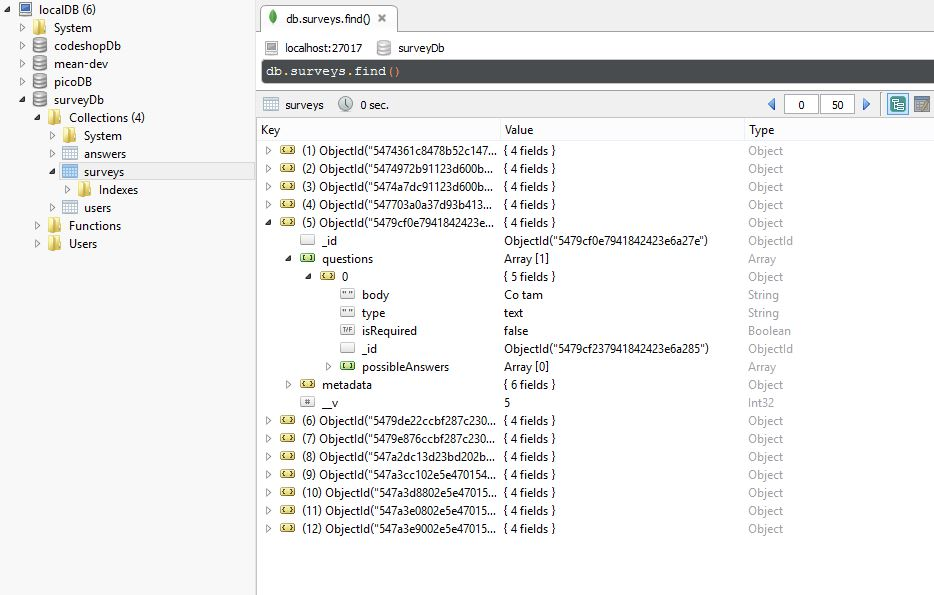
\includegraphics{obrazy/mongo}}
\caption{Struktura danych w~bazie MongoDB}
\end{center}
\end{figure}

\subsubsection{Mongoose}
Biblioteka Mongoose pozwala na ustandaryzowanie dostępu do bazy danych MongoDB. Generalnie, do MongoDB użytkownik może zapisać jakiekolwiek dane, nie istnieje żaden natywny sposób ograniczania lub walidacji wprowadzanych danych. Z~tego powodu powstała właśnie biblioteka Mongoose, w~której programista może zdefiniować strukturę kolekcji i~przy zapisywaniu danych do bazy przeprowadzana jest ich walidacja.
\par Listing 2. pokazuje sposób deklarowania struktury pojedynczej kolekcji bazy MongoDB z użyciem biblioteki Mongoose.

\begin{lstlisting}[caption=Przykład definicji struktury kolekcji w~bibliotece Mongoose ]
var surveySchema = mongoose.Schema({
  metadata: {
    userId: {
      type: mongoose.Schema.Types.ObjectId,
      required: true
    },
    title: {
      type: String,
      required: true
    },
    description: String,
    status: {
      type: String,
      enum: ['draft', 'inProgress', 'finished']
    },
    answerCount: Number,
    surveyCode: {
      type: String,
      unique: true
    }
  },
  questions: [questionSchema]
});
\end{lstlisting}

\subsubsection{Angular.JS}
Angular.JS jest frameworkiem frontendowym umożliwiającym tworzenie aplikacji w~stylu Single Page Application. Angular dzięki zastosowaniu wzorca MVC pozwala w~efektywny sposób oddzielić logikę aplikacji od widoku HTML. Najważniejszą funkcją Angulara jest dwukierunkowe wiązanie danych, która redukuje ilość kodu napisanego w~trakcie uwalniania backendu serwera z~odpowiedzialności za szablony. Szablony są stworzone w~prostym HTMLu zgodnie z~danymi zawartymi w~zakresie (scope) zdefiniowanym przez model. Serwis \$scope w~Angular wyłapuje zmiany w~modelu i~modyfikuje HTML w~widoku poprzez kontroler. Podobnie, wszelkie zmiany w~widoku widać w~modelu. To pozwala ominąć potrzebę aktywnego manipulowania DOMu i~ułatwia samodzielne i~szybkie tworzenie aplikacji internetowych. Angular wyłapuje zmiany w~modelach przez porównanie wartości z~wartościami zgromadzonymi we wcześniejszym procesie dirty-checking.

\subsubsection{Inne technologie}
Oprócz wymienionych wyżej technologii w~projekcie użytych zostało więcej dodatkowych bibliotek przydatnych przy realizacji pomniejszych zadań. Każda z~niżej wymienionych technologii jest dostępna na licencji MIT.

\begin{itemize}
\item Express.js - lekki framework dla Node.js ułatwiający stworzenie rozbudowanej aplikacji internetowej.
\item Twitter Bootstrap 3.0 - framework frontendowy zawierający gotowe arkusze stylów, ułatwiający szybkie zbudowanie aplikacji o~atrakcyjnym interfejsie.
\item Chart.JS - Biblioteka do rysowania wykresów na stronie HTML. Wykorzystuje znaczniki <canvas> wprowadzone w~HTML5.
\item passport.js - Moduł odpowiedzialny za obsługę uwierzytelniania i~autoryzacji użytkowników systemu oraz za obsługę sesji HTTP.
\item Lodash.js - Biblioteka ,,ogólnego użytku", dostarcza wielu przydatnych funkcji, jak wydajna obsługa kolekcji.
\item Nodemailer - Moduł odpowiedzialny za wysyłanie emaili do użytkowników. W~aplikacji wykorzystywany przy wysyłaniu linków aktywacyjnych do nowo powstałch kont.
\end{itemize}

\subsection{Diagram klas}
Język JavaScript, w~jakim wykonana została zarówno część serwerowa, jak i~kliencka, nie wymaga od programisty wykorzystywania klas i~obiektów. Jednak w~celu lepszej skalowalności zaleca się, aby w~większych aplikacjach używać podejścia obiektowego. W~obecnym etapie rozwoju języka JavaScript nie istnieje niestety kontrola typów, co znacznie utrudnia pracę, ale w~standardzie EcmaScript 6~planowane jest jej wprowadzenie.
\par W~części serwerowej aplikacji zdefiniowano kilka klas, których struktura widoczna jest na Rysunku 11.

\begin{figure}[H]
\begin{center}
\scalebox{0.7}{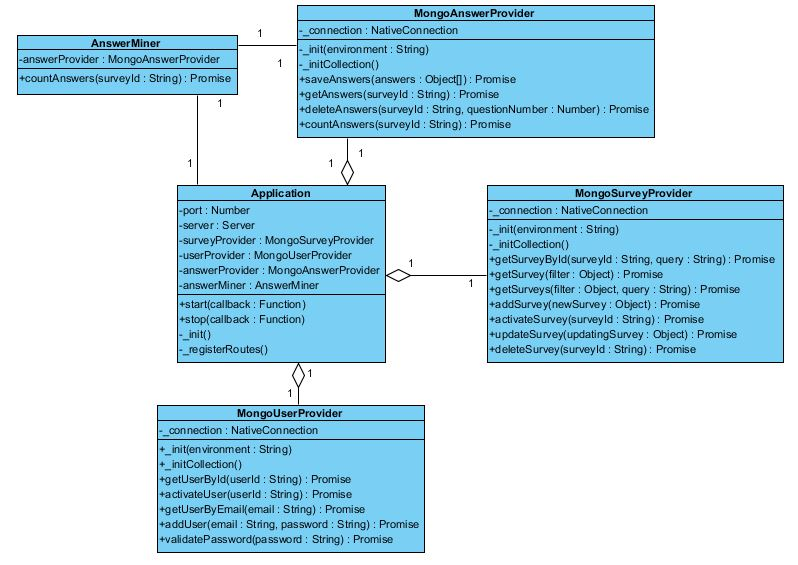
\includegraphics{obrazy/klasy}}
\caption{Diagram klas części serwerowej}
\end{center}
\end{figure}

\par Centralną klasą, odpowiedzialną za odpowiedzi na zapytania HTTP klientów, jest klasa Application. W~metodzie \texttt{\_registerRoutes()} inicjowana jest tablica routingu, czyli jakie adresy url są widoczne dla klientów i~jak są one obsługiwane. Klasa po wywołaniu funkcji \texttt{start()} tworzy serwer HTTP na zdefiniowanym w~konstruktorze porcie, na który przyjmowane są zapytania od klientów.

\par Klasy \texttt{MongoSurveyProvider, MongoAnswerProvider, MongoUserProvider} odpowiedzialne są za kontakt aplikacji z~serwerem bazy danych. Są one swoistym wrapperem na bibliotekę Mongoose i~dostarczają funkcji, za pomocą których programista może pobrać z~bazy danych interesujące go informacje.

\par Klasa \texttt{AnswerMiner} jest pomocniczą klasą, która jest odpowiedzialna za wstępne przetworzenie danych o~wynikach ankiet do struktury wymaganej przez bibliotekę Chart.js odpowiadającą za rysowanie wykresów.

\subsection{API}
W celu umożliwienia komunikacji między stroną kliencką a~serwerem, na serwerze zdefiniowano REST'owe API, do którego można wysyłać zapytania typu HTTP. API dostarcza możliwości pobierania oraz manipulowania danymi z~bazy danych. Definiuje również ścieżki dostępu do fragmentów stron HTML, które później są dynamicznie renderowane przez Angulara. Na Listingu 3. pokazano sposób definiowania tablicy routingu w~serwerze Node.js.
\begin{lstlisting}[caption=Definicja routingu w~Node.js ]
  router.route('/api/surveys')
    .get(hasAccess, surveys.getSurveys)
    .post(hasAccess, surveys.addSurvey);

  router.route('/api/surveys/:surveyId')
    .get(hasAccess, surveys.getSurveyById)
    .put(hasAccess, surveys.updateSurvey)
    .delete(hasAccess, surveys.deleteSurvey);

  router.route('/api/surveys/:surveyId/activate')
    .post(hasAccess, surveys.activateSurvey);

  router.route('/api/answers')
    .post(respond.saveAnswer);

  router.route('/api/answers/:surveyId')
    .get(respond.getAnswers)
    .post(respond.deleteAnswers);

  router.route('/api/code/:surveyCode')
    .get(surveys.getSurveyByCode);

  router.route('/')
    .get(views.index);


  router.route('/login')
    .get(auth.loginView)
    .post(passport.authenticate('local-login'));

  router.route('/signup')
    .get(auth.signupView)
    .post(passport.authenticate('local-signup'));

  router.route('/activation')
    .get(isLoggedIn, auth.activateUser);

  router.route('/profile')
    .get(isActive,views.profile);

  router.route('/survey/:surveyCode')
    .get(respond.surveyView);

  router.route('/partials/:filename')
    .get(views.partials);

  router.route('/partials/directives/:filename')
    .get(isLoggedIn,views.directive);

  router.route('/logout')
    .get(auth.logout);

  app.use('/', router);
\end{lstlisting}

Obiekt typu Router definiuje konkretną ścieżkę HTTP, a~następnie przypisuje jej obsługiwane funkcje (GET, POST, PUT, DELETE). Jeśli w~argumencie przekazanych jest więcej funkcji, wykonywane są one jedna po drugiej. W~tym przypadku w~wielu miejscach sprawdzane jest najpierw, czy użytkownik wykonujący zapytanie do serwera jest zalogowany (funkcja \texttt{hasAccess}), a~potem dopiero wykonuje właściwą część zapytania.
\par Na szczególną uwagę zasługują ścieżki zaczynające się przedrostkiem \texttt{/partials}. Wysyłają one do klienta fragmenty widoków HTML, które następnie Angular.JS wstawia w~odpowiednie miejsca na stronie.
\par Dane z~serwera są wysyłane do klienta w~postaci dokumentów JSON.

\subsubsection{/api/surveys}
Metody:
\begin{itemize}
\item \textbf{GET} \\ Zwraca dane o~ankietach 
\item \textbf{POST} \\ Dodaje do bazy danych nową ankietę. \\ Parametry:
	\begin{itemize}
	\item title \{String\} - tytuł ankiety
	\item description \{String\} - opis ankiety
	\end{itemize}
\end{itemize}

\subsubsection{/api/surveys/\{surveyId\}}
Metody:
\begin{itemize}
\item \textbf{GET} \\ Zwraca dane o~ankiecie o~podanym identyfikatorze. \\ Parametry:
	\begin{itemize}
	\item surveyId \{String\} - identyfikator ankiety
	\end{itemize}
\item \textbf{PUT} \\ Modyfikuje ankietę o~podanym ID. \\ Parametry:
	\begin{itemize}
	\item surveyId \{String\} - identyfikator ankiety
	\item survey \{Object\} - zmodyfikowana ankieta
	\end{itemize}

\item \textbf{DELETE} \\ Usuwa ankietę o~podanym ID. \\ Parametry:
	\begin{itemize}
	\item surveyId \{String\} - identyfikator ankiety
	\end{itemize}
\end{itemize}

\subsubsection{/api/surveys/\{surveyId\}/activate}
Metody:
\begin{itemize}
\item \textbf{POST} \\ Zmienia status ankiety o~podanym ID na 'inProgress'. \\ Parametry:
	\begin{itemize}
	\item surveyId \{String\} - identyfikator ankiety
	\end{itemize}

\end{itemize}

\subsubsection{/api/answers}
Metody:
\begin{itemize}
\item \textbf{POST} \\ Zapisuje pojedynczy zbiór odpowiedzi do podanej ankiety. \\ Parametry:
	\begin{itemize}
	\item answers \{String\} - zbiór odpowiedzi do konkretnrj ankiety. Zawiera w~sobie ID ankiety
	\end{itemize}

\end{itemize}

\subsubsection{/api/answers/\{surveyId\}}
Metody:
\begin{itemize}
\item \textbf{GET} \\ Pobiera informacje o~odpowiedziach w~ankiecie o~podanym ID. \\ Parametry:
	\begin{itemize}
	\item surveyId \{String\} - identyfikator ankiety
	\end{itemize}
\item \textbf{POST} \\ Usuwa odpowiedzi na konkretne pytanie z~podanej ankiety. \\ Parametry:
	\begin{itemize}
	\item surveyId \{String\} - ID ankiety
	\item questionNumber \{Number\} - numer pytania
	\end{itemize}

\end{itemize}

\subsubsection{/api/code/\{surveyCode\}}
Metody:
\begin{itemize}
\item \textbf{GET} \\ Pobiera informacje o~ankiecie o~podanym kodzie ankiety. \\ Parametry:
	\begin{itemize}
	\item surveyCode \{String\} - kod ankiety
	\end{itemize}

\end{itemize}

\subsection{Komunikacja serwera HTTP z~bazą danych}
Poniżej opisane zostały klasy pełniące funkcje dostępu do bazy danych.

\subsubsection{MongoSurveyProvider}
Klasa odpowiedzialna za dostep do danych z~kolekcji \texttt{surveys}. \\
Metody:
\begin{center}
\begin{table}[H]
\caption{Opis funkcji klasy MongoSurveyProvider}
  \begin{tabular}{| l| l|}%left i~center wyrownanie
    \hline
    Typ zwracany & Opis \\ \hline \hline
  	q.Promise	&	\textbf{getSurveyById}(\{String\} surveyId, \{String\} query) \\
 &  Pobiera z~bazy danych ankietę i~przekazuje ją do funkcji zwrotnej \\ 
 & Parametry: \\
 & surveyId - identyfikator ankiety \\ 
 & query - ciąg znaków informujący jakie dane ankiety wyciągnąć \\ \hline

q.Promise	&	\textbf{getSurvey}(\{Object\} filter, \{String\} query) \\
 &  Pobiera z~bazy danych tablicę ankiet spełniających odpowiednie  \\ & kryteria filtrowania \\ 
 & Parametry: \\
 & filter - kryteria filtrowania \\ 
 & query - ciąg znaków informujący jakie dane ankiety wyciągnąć \\ \hline
   
q.Promise	&	\textbf{addSurvey}(\{Object\} newSurvey) \\
 &  Dodaje do bazy danych nową ankietę.\\ 
 & Parametry: \\
 & newSurvey - ankieta zapisywana do bazy \\ 
 \hline

q.Promise	&	\textbf{activateSurvey}(\{String\} surveyId) \\
 &  Aktywuje ankietę o~podanym ID.\\ 
 & Parametry: \\
 & surveyId - identyfikator ankiety \\ 
 \hline
   
q.Promise	&	\textbf{updateSurvey}(\{String\} surveyId, \{Object\} updatingSurvey) \\
 &  Aktualizuje dane ankiety o~podanym ID. \\ 
 & Parametry: \\
 & surveyId - identyfikator ankiety \\ 
 & updatingSurvey - zaktualizowana ankieta \\ \hline

q.Promise	&	\textbf{deleteSurvey}(\{String\} surveyId) \\
 &  Usuwa ankietę o~podanym ID.\\ 
 & Parametry: \\
 & surveyId - identyfikator ankiety \\ 
 \hline
  \end{tabular}
\end{table}
\end{center}

\par Na lisitingu 4. pokazano przykład użycia metody \texttt{getSurvey} w celu pobrania z bazy i wysłania do użytkownika ankiety o podanym kodzie.

\begin{lstlisting}[caption=Przykład użycia metody \texttt{getSurvey} ]
surveyProvider.getSurvey({
  "metadata.surveyCode": req.params.surveyCode
}).then(function(result) {
  MessageSender.sendJsonObject(res, result);
});
\end{lstlisting}

\subsubsection{MongoAnswerProvider}
Klasa odpowiedzialna za dostęp do kolekcji \texttt{answers}. \\ 
Metody: 
\begin{center}
\begin{table}[H]
\caption{Opis funkcji klasy MongoAnswerProvider}
  \begin{tabular}{| l| l|}%left i~center wyrownanie
    \hline
    Typ zwracany & Opis \\ \hline \hline
  	q.Promise	&	\textbf{saveAnswers}(\{Object[ ]\} answers) \\
 &  Dodaje do bazy danych odpowiedzi do konkretnej ankiety. \\ 
 & Parametry: \\
 & answers - tablica obiektów opisujących odpowiedzi do ankiety \\ 
 \hline

q.Promise	&	\textbf{getAnswers}(\{String\} surveyId) \\
 &  Pobiera z~bazy danych odpowiedzi do konkretnej ankiety \\ 
 & Parametry: \\
 & surveyId - identyfikator ankiety \\ 
\hline
   
q.Promise	&	\textbf{deleteAnswers}(\{String\} surveyId, \{Number\} questionNumber) \\
 &  Usuwa z~bazy danych odpowiedzi dotyczące zadanego pytania \\ &  w~ankiecie.\\ 
 & Parametry: \\
 & surveyId - identyfikator ankiety \\ 
 & questionNumber - numer pytania \\
 \hline

q.Promise	&	\textbf{countAnswers}(\{String\} surveyId) \\
 &  Oblicza  ile odpowiedzi padło w~danej ankiecie na dane pytanie.\\ 
 & Parametry: \\
 & surveyId - identyfikator ankiety \\ 
 \hline
 
  \end{tabular}
\end{table}
\end{center}

\par Na lisitingu 5. pokazano przykład użycia metody \texttt{saveAnswers}, w którym do bazy danych zapisywane są odpowiedzi do ankiety przesłane przez respondenta.

\begin{lstlisting}[caption=Przykład użycia metody \texttt{saveAnswers} ]
answerProvider.saveAnswers(answers)
  .then(function (result) {
    MessageSender.sendJsonObject(res, result);
  }, function (err) {
    MessageSender.sendDatabaseError(res, err);
  });
\end{lstlisting}

\newpage
\subsubsection{MongoUserProvider}
Klasa odpowiedzialna za dostęp do kolekcji \texttt{users} \\ 
Metody:

\begin{center}
\begin{table}[H]
\caption{Opis funkcji klasy MongoUserProvider}
  \begin{tabular}{| l| l|}%left i~center wyrownanie
    \hline
    Typ zwracany & Opis \\ \hline \hline
  	q.Promise	&	\textbf{getUserById}(\{String\} userId, \{String\} query) \\
 &  Pobiera dane o~użytkowniku o~podanym identyfikatorze. \\ 
 & Parametry: \\
 & userId - ID użytkownika \\
 & query - ciąg znaków informujący jakie dane użytkownika \\ & wyciągnąć \\ 
 \hline

q.Promise	&	\textbf{getUserByEmail}(\{String\} email) \\
 &  Pobiera z~bazy danych dane użytkownika o~podanym emailu.\\ 
 & Parametry: \\
 & email - adres email użytkownika\\ 
\hline
   
q.Promise	&	\textbf{activateUser}(\{String\} activationCode) \\
 &  Aktywuje konto użytkownika.\\ 
 & Parametry: \\
 & activationCode - kod aktywacyjny użytkownika \\ 
 \hline

q.Promise	&	\textbf{addUser}(\{String\} email, \{String\} password) \\
 &  Dodaje do bazy danych nowego użytkownika.\\ 
 & Parametry: \\
 & email - adres email nowego użytkownika \\
 & password - hasło nowego użytkownika \\ 
 \hline

Boolean	&	\textbf{validatePassword}(\{String\} password) \\
 &  Sprawdza poprawność wprowadzonego hasła.\\ 
 & Parametry: \\
 & password - hasło  użytkownika \\ 
 \hline
 
  \end{tabular}
\end{table}
\end{center}

\par Na lisitingu 6. pokazano przykład użycia metody \texttt{getUserByEmail} podczas operacji rejestrowania użytkownika w serwisie.

\newpage
\begin{lstlisting}[caption=Przykład użycia metody \texttt{getUserByEmail} ]
userProvider.getUserByEmail(email)
  .then(function(user) {
    if(user) {
      return done(null, false, req.flash('signupMessage', Message.EMAIL_TAKEN.en));
    } else {
      userProvider.addUser(email, password, function(err, newUser) {
        if (err)
          throw err;
        return done(null, newUser);
      });
    }
  }, function(err) {
    return done(err);
  });
\end{lstlisting}

\newpage
\section{Testowanie}
W trakcie pisania aplikacji częściowo wprowadzona została koncepcja TDD (ang. \textit{Test Driven Development}). Napisane zostały testy jednostkowe dla funkcji dostępu do bazy danych oraz testy REST'owego API. Zdefiniowano również szereg scenariuszy testowych dla testów funkcjonalnych.
\par Poniżej przedstawiono tylko niektóre testy, które zostały przeprowadzone na aplikacji.

\subsection{Tworzenie nowej ankiety}
\textbf{Cel testu}: testowanie poprawnego tworzenia ankiety. \\
\textbf{Scenariusz (kroki testowe):}
\begin{center}

  \begin{tabular}{| l| l|}
    \hline
    
 \textbf{Akcje użytkownika} &  \textbf{Odpowiedź systemu} \\  \hline
1. Przejście na stronę logowania. & 2. Wyświetlenie strony logowania. \\ 
3. Wpisanie poprawnych danych logowania. & 4. Przekierowanie na stronę  \\ 
& użytkownika \\ 
5. Naciśnięcie przycisku ,,Create survey" & 6. Wyświetlenie strony do wpisania \\ & danych ankiety \\
7. Wpisanie danych ankiety i~zatwierdzenie. & 8. Przejście na stronę z~ \\ &  podstawowymi danymi ankiety. \\
\hline
 
  \end{tabular}
\end{center}

\textbf{Ocena testu: } Pozytywna

\subsection{Edycja pytań ankiety}

\textbf{Cel testu}: testowanie poprawnego edytowania pytań. \\
\textbf{Scenariusz (kroki testowe):}
\begin{center}
  \begin{tabular}{| l| l|}
    \hline
    
 \textbf{Akcje użytkownika} &  \textbf{Odpowiedź systemu} \\  \hline
1. Przejście na stronę logowania. & 2. Wyświetlenie strony logowania. \\ 
3. Wpisanie poprawnych danych logowania. & 4. Przekierowanie na stronę  \\ 
& użytkownika \\ 
5. Wybranie jednej z~ankiet widocznych & 6. Przejście na stronę z~ \\  na liście ankiet &  podstawowymi danymi ankiety. \\
7. Przejście do zakładki ,,Edit questions". & 8. Wyświetlenie widoku edycji \\ & pytań. \\
9. Wciśnięcie przycisku ,,Add new question". & 10. Dodanie na stronie nowego \\ & pytania. \\
11. Modyfikacja danych pytania. & 12. Zapisanie zmodyfikowanego  \\ & pytania. \\
\hline
 
  \end{tabular}
\end{center}

\textbf{Ocena testu: } Pozytywna

\newpage
\subsection{Analiza zebranych wyników}

\textbf{Cel testu}: testowanie poprawnego zliczania odpowiedzi. \\
\textbf{Scenariusz (kroki testowe):}
\begin{center}
  \begin{tabular}{| l| l|}
    \hline
    
 \textbf{Akcje użytkownika} &  \textbf{Odpowiedź systemu} \\  \hline
1. Przejście na stronę logowania. & 2. Wyświetlenie strony logowania. \\ 
3. Wpisanie poprawnych danych logowania. & 4. Przekierowanie na stronę  \\ 
& użytkownika \\ 
5. Wybranie jednej z~ankiet widocznych & 6. Przejście na stronę z~ \\  na liście ankiet &  podstawowymi danymi ankiety. \\
7. Przejście do zakładki ,,Sharing". & 8. Wyświetlenie widoku  \\ & udostępniania ankiety. \\
9. Wciśnięcie przycisku ,,Activate survey". & 10. Wygenerowanie kodu \\ & ankiety. \\
11. Przejście w~drugiej przeglądarce pod & 12. Wyświetlenie widoku ankiety  \\  wygenerowany adres. & z~możliwością odpowiedzi. \\
13. Oddanie głosu na konkretne pytanie & 14. Wyświetlenie komunikatu \\  i~wysłanie odpowiedzi. &  o~poprawnym zagłosowaniu. \\
15. W~panelu autora ankiety przejście do  & 16. Wyświetlenie widoku analizy  \\ zakładki ,,Analysis". & wyników. \\
17. Naciśnięcie przycisku ,,Get answers". & 18. Wyświetlenie wykresu  \\ &  pokazującego jedną odpowiedź \\ & oddaną w~drugiej przeglądarce. \\
\hline
 
  \end{tabular}
\end{center}

\textbf{Ocena testu: } Pozytywna

\subsection{Kontrola jednokrotnego głosowania}

\textbf{Cel testu}: testowanie oddawania tylko jednego głosu przez respondenta. \\
\textbf{Scenariusz (kroki testowe):}
\begin{center}
  \begin{tabular}{| l| l|}
    \hline
    
 \textbf{Akcje użytkownika} &  \textbf{Odpowiedź systemu} \\  \hline
1. Przejście na stronę logowania. & 2. Wyświetlenie strony logowania. \\ 
3. Wpisanie poprawnych danych logowania. & 4. Przekierowanie na stronę  \\ 
& użytkownika \\ 
5. Wybranie jednej z~ankiet widocznych & 6. Przejście na stronę z~ \\  na liście ankiet &  podstawowymi danymi ankiety. \\
7. Przejście do zakładki ,,Sharing". & 8. Wyświetlenie widoku  \\ & udostępniania ankiety. \\
9. Wciśnięcie przycisku ,,Activate survey". & 10. Wygenerowanie kodu \\ & ankiety. \\
11. Przejście w~drugiej przeglądarce pod & 12. Wyświetlenie widoku ankiety  \\  wygenerowany adres. & z~możliwością odpowiedzi. \\
13. Oddanie głosu na konkretne pytanie & 14. Wyświetlenie komunikatu \\  i~wysłanie odpowiedzi. &  o~poprawnym zagłosowaniu. \\
15. Zamknięcie przeglądarki i~ponowne & Wyświetlenie komunikatu  \\  jej otworzenie, przejście pod wygenerowany & o~poprawnym zagłosowaniu. \\  adres. & \\
\hline
 
  \end{tabular}
\end{center}

\textbf{Ocena testu: } Pozytywna

\newpage
\section {Wdrożenie}

\subsection{Node.js}
Pierwszym krokiem do wdrożenia aplikacji Code-Shop jest zainstalowanie platformy \textit{Node.js}. Aplikacja została stworzona w~wersji \textit{v0.10.33} platformy. Node.js jest biblioteką wieloplatformową i~może być zainstalowany w~większości popularnych systemów operacyjnych.
\par Rysunek 12. pokazuje dostępne sposoby pobierania Node.js.

\begin{figure}[H]
    \centering
    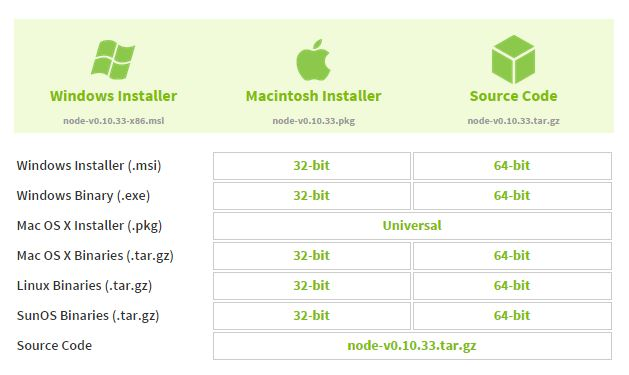
\includegraphics[width=\linewidth]{obrazy/node}
    \caption{Strona internetowa Node.js umożliwiająca pobranie środowiska}
\end{figure} 

\subsubsection{Windows}
Aby zainstalować \textit{Node.js} na systemie operacyjnym \textit{Windows} wystarczy przejść na stronę \textit{http://nodejs.org/download/}, skąd można pobrać przeznaczone dla tego systemu instalatory (.msi lub .exe). Następnie należy postępować zgodnie z~instrukcjami tegoż instalatora, co spowoduje zainstalowanie środowiska w systemie operacyjnym.

\subsubsection{Linux}
Poniżej przedstawiono instrukcję instalacji dla dwóch dystrybucji Linuxa: Debian i~Ubuntu. Jest poprawna również dla dystrybucji opartych na tych dwóch, takich jak Linux Mint, Linux Mint Debian Edition, elementaryOS. \\
Pierwszym krokiem jest skonfigurowanie repozytoriów Node.js:
\begin{lstlisting}
curl -sL https://deb.nodesource.com/setup | bash -
\end{lstlisting}

Następnym, ostatnim krokiem jest zaistalowanie środowiska za pomocą menadżera pakietów \textit{apt-get}:
\begin{lstlisting}
apt-get install -y nodejs
\end{lstlisting}

Powyższe kroki odnoszą się do systemu Debian. Na Ubuntu proces instalacji jest praktycznie identyczny, należy tylko dodać komendę \texttt{sudo}.

\subsection{Nginx}
\subsubsection{Windows}
W celu zainstalowania serwera na Windowsie, należy pobrać ze strony \\ http://nginx.org/en/download.html plik .zip zawierający serwer Nginx. Następnie należy zmodyfikować konfigurację serwera w~sposób opisany w~punkcie 6.2.3. Aby uruchomić serwer jako serwis, należy przejść w~konsoli do katalogu, gdzie został wypakowany, a~następnie wpisać komendę:
\begin{lstlisting}
start nginx
\end{lstlisting}

\subsubsection{Linux}
Aby zainstalować serwer Nginx na Linuksie (Debian/Ubuntu) należy zaktualizować repozytoria pakietów komendą
\begin{lstlisting}
apt-get update
\end{lstlisting}
a następnie zainstalować komendą
\begin{lstlisting}
apt-get install nginx
\end{lstlisting}
Po tym kroku należy zmodyfikować konfigurację serwera (domyślnie znajduje się w~pliku /etc/nginx/conf/nginx.conf) w~sposób opisany w~punkcie 6.2.3, po czym zrestartować serwer komendą
\begin{lstlisting}
service nginx restart
\end{lstlisting}

\subsubsection{Konfiguracja serwera}
W pliku konfiguracyjnym serwera Nginx (nginx.conf) w~bloku \texttt{http} należy wprowadzić nastepujące dane:
\begin{lstlisting}
server {
  listen 80;
  server_name {nazwa_serwera};
  rewrite ^ https://$server_name$request_uri;
}
server {
  listen       443;
  ssl on;
  server_name  {nazwa serwera};

  ssl_certificate  {sciezka do certyfikatu SSL};
  ssl_certificate_key {sciezka do klucza SSL};

  location / {
    proxy_pass http://localhost:7070;
    proxy_set_header Upgrade $http_upgrade;
    proxy_set_header Connection 'upgrade';
    proxy_set_header Host $host;
  }
\end{lstlisting}

\par Przykładowa konfiguracja została przedstawiona poniżej.

\begin{lstlisting}
server {
  listen 80;
  server_name example.com;
  rewrite ^ https://$server_name$request_uri;
}
server {
  listen       443;
  ssl on;
  server_name  example.com;

  ssl_certificate  /etc/ssl/server.crt;
  ssl_certificate_key /etc/ssl/server.key;

  location / {
    proxy_pass http://localhost:7070;
    proxy_set_header Upgrade $http_upgrade;
    proxy_set_header Connection 'upgrade';
    proxy_set_header Host $host;
  }
\end{lstlisting}

\subsection{MongoDB}
\subsubsection{Windows}
Baza danych MongoDB dla systemu Windows przeznaczona jest dla różnych architektur, więc w~pierwszej kolejności należy zidentyfikować jaki typ systemu jest zainstalowany na danym komputerze. Następnie należy przejść na stronę pobierania MongoDB (http://www.mongodb.org/downloads) i~pobrać odpowiednią wersję bazy (2.6.4). Kolejnym krokiem jest samo zainstalowanie MongoDB, które polega na postępowaniu według instrukcji instalatora.
\par Rysunek 13. pokazuje sposoby pobierania MongoDB.
\begin{figure}[H]
    \centering
    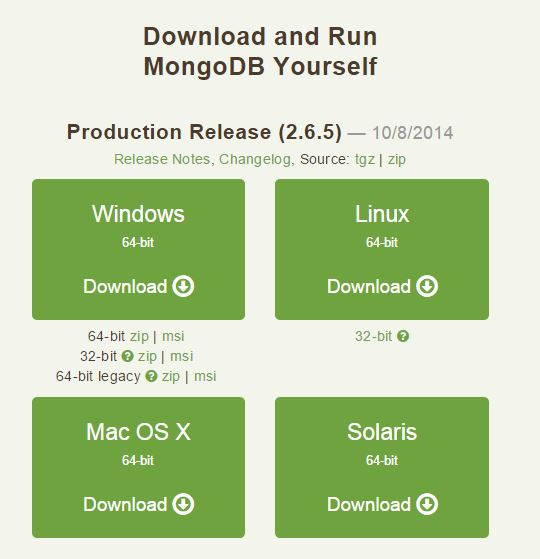
\includegraphics[width=\linewidth]{obrazy/mongoWdr}
    \caption{Strona internetowa MongoDB umożliwiająca pobranie bazy danych}
\end{figure} 
Po zainstalowaniu bazy danych należy uruchomić ją jako serwis. W~tym celu należy uruchomić wiersz poleceń systemu Windows jako administrator, a~następnie postępować wg następujących kroków: \\
\begin{enumerate}
\item Stwórz katalogi na pliki bazy danych oraz na logi.
\begin{lstlisting}
mkdir c:\data\db
mkdir c:\data\log
\end{lstlisting}
\newpage
\item Stwórz plik konfiguracyjny za pomocą następujących poleceń:
\begin{lstlisting}
echo logpath=c:\data\log\mongod.log> "C:\Program Files\MongoDB 2.6 Standard\mongod.cfg"
echo dbpath=c:\data\db>> "C:\Program Files\MongoDB 2.6 Standard\mongod.cfg"
\end{lstlisting}

\item Utwórz serwis MongoDB.
\begin{lstlisting}
sc.exe create MongoDB binPath= "\"C:\Program Files\MongoDB 2.6 Standard\bin\mongod.exe\" --service --config=\"C:\Program Files\MongoDB 2.6 Standard\mongod.cfg\"" DisplayName= "MongoDB 2.6 Standard" start= "auto"
\end{lstlisting}
Jeśli komenda zakończy się sukcesem powinien pojawić się następujący komunikat:
\begin{lstlisting}
[SC] CreateService SUCCESS
\end{lstlisting}

\item Uruchom serwis MongoDB
\begin{lstlisting}
net start MongoDB
\end{lstlisting}

\end{enumerate}

\par Po wykonaniu powyższego procesu w~systemie Windows pracuje serwis MongoDB, z~którego będzie korzystać aplikacja.

\subsubsection{Linux}
Aby zainstalować MongoDB na systemie typu Linux należy: 
\begin{enumerate}
\item Zaimportować klucz publiczny przez menadżer pakietów systemu:
\begin{lstlisting}
sudo apt-key adv --keyserver hkp://keyserver.ubuntu.com:80 --recv 7F0CEB10
\end{lstlisting}

\item Stworzyć plik \texttt{.list} dla MongoDB:
\begin{lstlisting}
echo 'deb http://downloads-distro.mongodb.org/repo/ubuntu-upstart dist 10gen' | sudo tee /etc/apt/sources.list.d/mongodb.list
\end{lstlisting}

\item Zaktualizować lokalną bazę pakietów:
\begin{lstlisting}
sudo apt-get update
\end{lstlisting}

\item Zainstalować pakiety MongoDB:
\begin{lstlisting}
sudo apt-get install -y mongodb-org
\end{lstlisting}

\item Wystartować bazę danych jako serwis:
\begin{lstlisting}
sudo service mongod start
\end{lstlisting}
\end{enumerate}

Po wykonaniu tego kroku wystartowany został serwis MongoDB. Poniższa została przetestowana na dystrybucjach Ubuntu oraz Debian.



\subsection{Instalacja zależności projektowych}
Aby uruchomić projekt należy najpierw zainstalować wszystkie niezbędne biblioteki, z~których aplikacja będzie korzystać. Po przejściu do głównego katalogu, gdzie wypakowany został projekt, należy uruchomić następującą komendę:
\begin{lstlisting}
npm install
\end{lstlisting}
Komenda ta instaluje wszystkie biblioteki zapisane w~pliku \texttt{package.json}. Menadżer pakietów \texttt{npm} został zainstalowany razem z~Node.js. Instalacja zewnętrzych bibliotek wygląda tak samo na wszystkich systemach operacyjnych.

\subsection{Uruchomienie aplikacji}
Po przejściu przez wszytkie poprzednie kroki użytownik jest gotowy do uruchomienia aplikacji. Na początku należy ustawić zmienną systemową \texttt{NODE\_ENV} na wartość \texttt{production}. Najprostszą wersją jest uruchomienia aplikacji jest wpisanie w~terminalu następującej komendy:
\begin{lstlisting}
node app.js
\end{lstlisting}
będąc w~katalogu głównym projektu. Niestety po zamknięciu terminala proces zostanie zamknięty. Aby uruchomić proces jako serwis najlepiej użyć biblioteki \texttt{forever}. Instalacja biblioteki odbywa się za pomocą poznanego wcześniej menadżera pakietów \texttt{npm}. Aby zainstalować bibliotekę \texttt{forever} należy w~terminalu wprowadzić następującą komendę:
\begin{lstlisting}
npm install forever -g
\end{lstlisting}
Opcja \texttt{-g} informuje, że biblioteka ma być zainstalowana globalnie. 
\\
Po zainstalowaniu forevera, będąc w~katalogu głównym projektu wprowadzić należy komendę:
\begin{lstlisting}
forever start app.js
\end{lstlisting}

\newpage
\section{Instrukcja użytkowania}
\subsection{Rejestracja w~serwisie}
Aby zarejestrować się w~systemie należy w~panelu rejestracji podać swój adres email oraz wpisać hasło do konta. Na podany adres wysłany zostanie link aktywacyjny, który należy kliknąć. Po zrobieniu tego użytkownik przeniesiony zostanie do strony logowania, gdzie za pomocą swoich danych będzie mógł wejść do serwisu. Widok ekranu rejestracji przedstawiony został na Rysunku 14.

\begin{figure}[H]
    \centering
    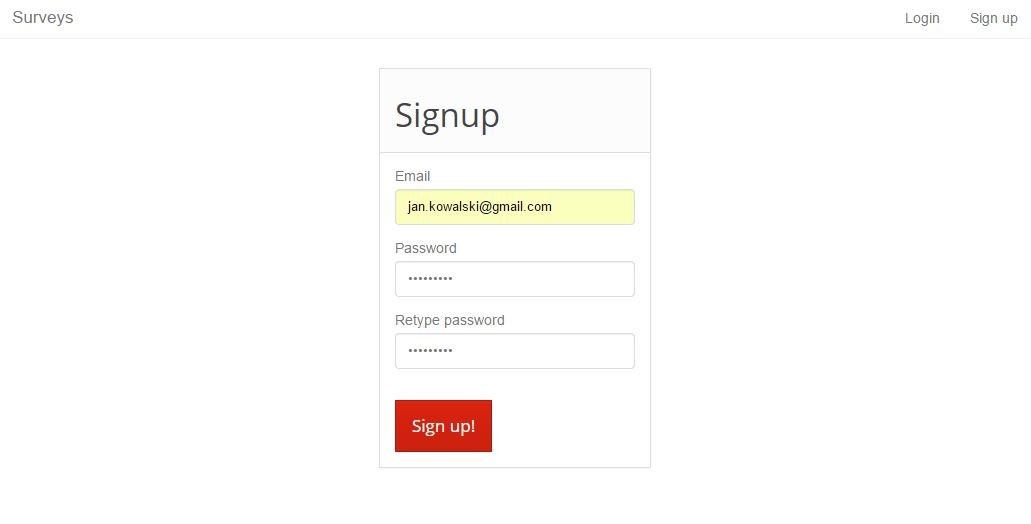
\includegraphics[width=\linewidth]{obrazy/register}
    \caption{Strona rejestracji użytkownika}
\end{figure} 

\subsection{Tworzenie i~edycja ankiety}
Po zalogowaniu użytkownik ma możliwość stworzenia nowej ankiety oraz edycji już istniejących. Schemat działania jest praktycznie taki sam, więc został opisany w~jednym punkcie. Aby stworzyć nową ankietę należy w~głównym widoku nacisnąć przycisk ,,Create survey", po czym wpisać tytuł i~opis ankiety. Kroki te pokazane są kolejno na Rysunkach 15. i 16.

\begin{figure}[H]
    \centering
    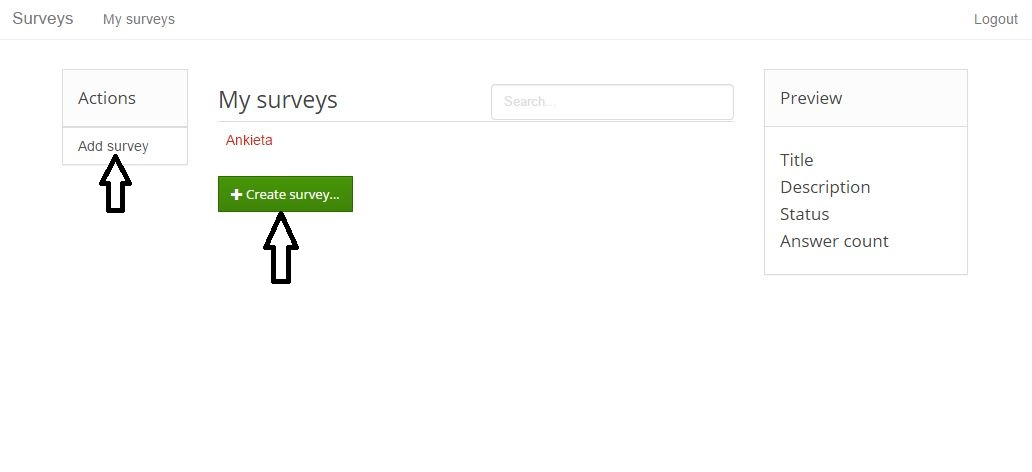
\includegraphics[width=\linewidth]{obrazy/newSurvey}
    \caption{Tworzenie nowej ankiety}
\end{figure} 

\begin{figure}[H]
    \centering
    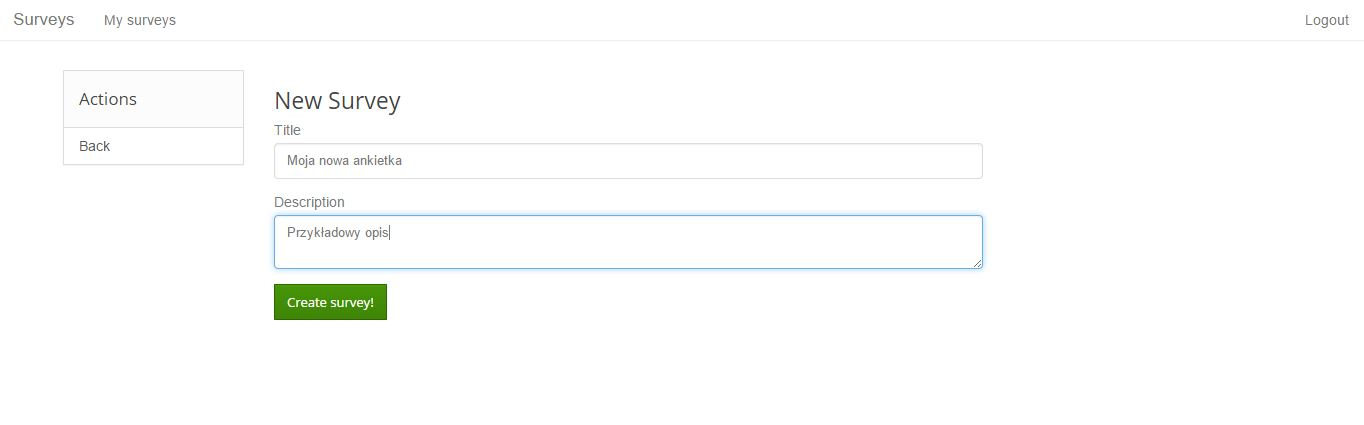
\includegraphics[width=\linewidth]{obrazy/edycjaBasic}
    \caption{Tworzenie nowej ankiety}
\end{figure} 

Następnie można przejść do edycji pytań. W~celu dodania nowego pytania należy nacisnąć przycisk ,,Add new question". Aby zmienić treść pytania należy na nie kliknąć i~wpisać nowy tekst, po czym zatwierdzić przyciskiem. Można zmienić typ pytania, zdefiniować, czy pytanie jest wymagane, oraz dodać możliwe odpowiedzi. Po jakiejkolwiek edycji pytania, dane ankiety są automatycznie zapisywane w~bazie danych.
\par Widok edycji pytań przedstawiony został na Rysunku 17.

\begin{figure}[H]
    \centering
    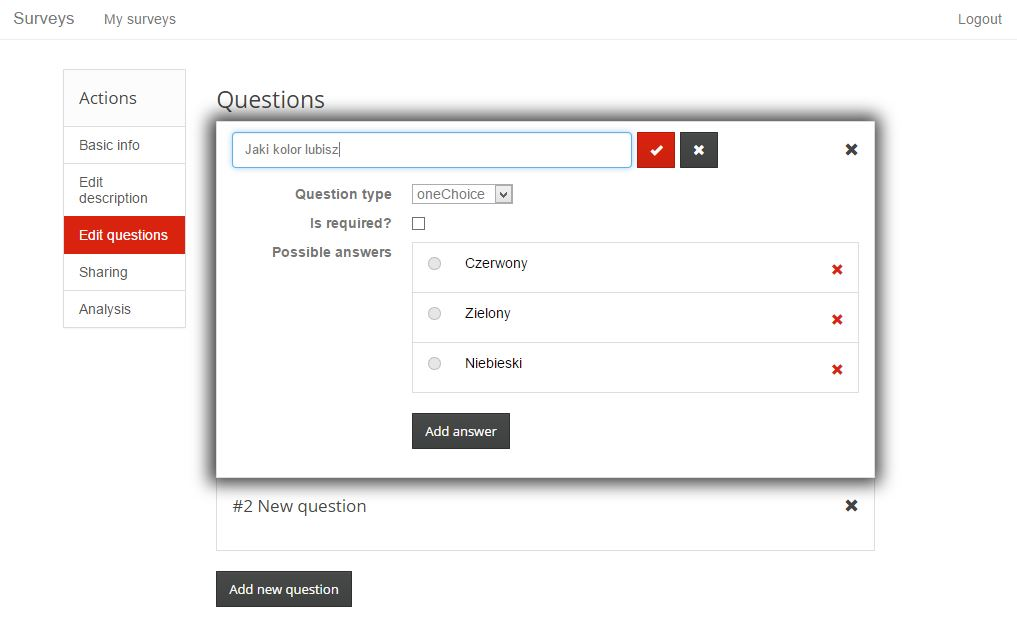
\includegraphics[width=\linewidth]{obrazy/edycjaPytan}
    \caption{Edycja pytań}
\end{figure} 

\subsubsection{Udostępnianie ankiety}
Aby udostępnić ankietę dla respondentów należy wygenerować link do ankiety. W~tym celu należy w~widoku ankiety przejść do zakładki ,,Sharing", a~następnie kliknąć przycisk ,,Activate survey". W~polu tekstowy pojawi się link do ankiety, który można rozesłać do respondentów.
\par Ekran udostępniania ankiety pokazany został na Rysunku 18.

\begin{figure}[H]
    \centering
    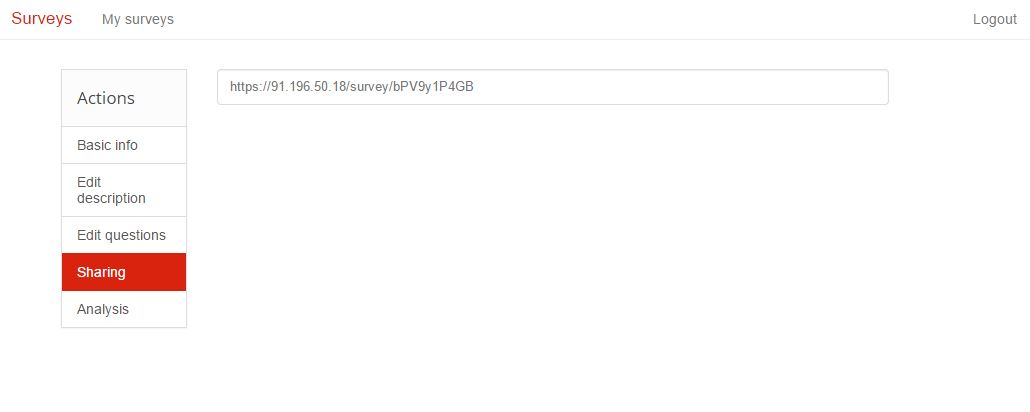
\includegraphics[width=\linewidth]{obrazy/sharing}
    \caption{Udostępnianie ankiety}
\end{figure} 

\subsubsection{Analiza wyników}
W celu przeprowadzenia analizy wyników ankiety należy w~widoku ankiety przejść do zakładki ,,Analysis". Następnie należy nacisnąć przycisk ,,Get answers". Po wykonaniu tej czynności powinny wygenerować się wykresy przedstawiające wyniki ankiety.
\par Przykładowa analiza wyników pokazana została na rysunku 19.

\begin{figure}[H]
    \centering
    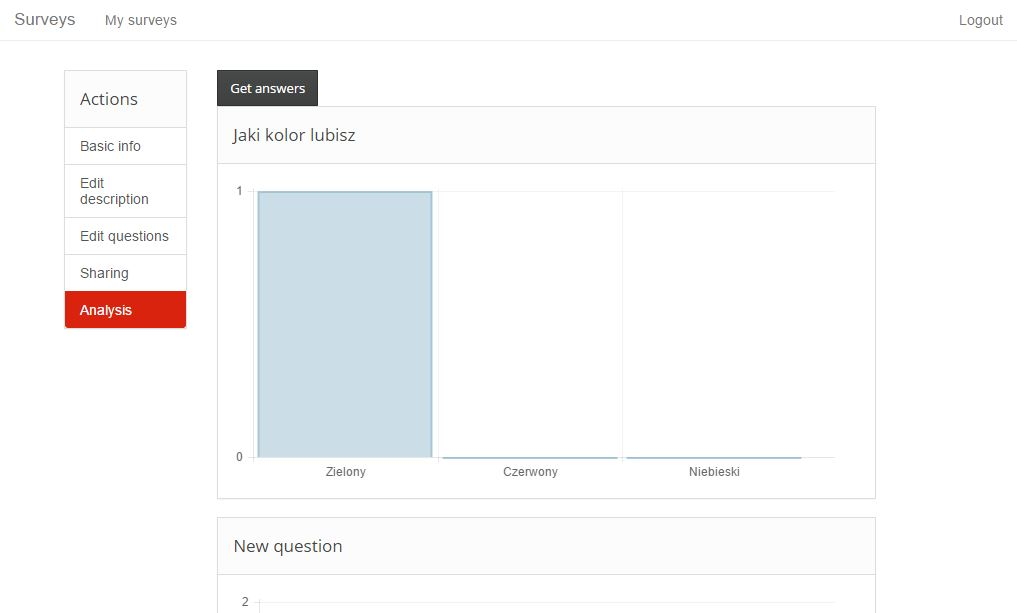
\includegraphics[width=\linewidth]{obrazy/analysis}
    \caption{Analiza ankiety}
\end{figure}

\newpage
\section{Podsumowanie i~wnioski}
Udało się zrealizować wszystkie niezbędne do działania systemu funkcjonalności. Funkcjonalności dodatkowe zostały pominięte w~podstawowej wersji serwisu, ale planowana jest ich implementacja w~przyszłych wersjach aplikacji.
\par Wybrane technologie, mimo stosunkowo młodego wieku, dobrze sprawdziły się w~implementacji projektu. Szczególnie baza MongoDB, ze względu na swoją prostotę, znacznie ułatwiła stworzenie struktury danych przetwarzanych przez aplikację. 
\par Zastosowanie koncepcji Single Page Application zwiększyło komfort korzystania z~serwisu. Jest to rozwiązanie znacznie szybsze od standardowego podejścia. Obserwując dzisiejszy rynek technologii internetowych można zauważyć znaczny wzrost popularności tego typu rozwiązań, przede wszystkim dzięki powstawaniu nowoczesnych frameworków do tego przeznaczonych, np. użytemu w~projekcie Angularowi.

\subsection{Perspektywy rozwoju aplikacji}
W kolejnych wersjach serwisu planowane jest zaimplementowanie dodatkowych funkcjonalności, przede wszystkim:
\begin{itemize}
\item Pobieranie wyników ankiety w~czasie rzeczywistym dzięki zastosowaniu technologii WebSockets,
\item Eksportowanie wyników ankiety do zewnętrznych plików (np. xlsx, csv).
\end{itemize}

Oprócz tego planowane jest rozwinięcie już istniejących funkcjonalności:
\begin{itemize}
\item Wprowadzenie większej liczby typów pytań (pytania macierzowe, skalowe).
\item Zwiększenie możliwości analizy wyników ankiety (np. tabelki).
\item Lepsza analiza odpowiedzi na pytania otwarte.
\end{itemize}

\subsection{Opis zawartości płyty CD}
Płyta CD dołączona do dokumentacji zawiera kod źródłowy projektu oraz elektroniczną wersję dokumentacji w formacie PDF. Kod źródłowy aplikacji umieszczony został w folderze ,,surveys", a dokumentacja w folderze ,,dokumentacja".

\newpage
\section*{Literatura}

\addcontentsline{toc}{section}{\protect\numberline{}Literatura}%
1. Ethan Brown, \textit{Web development with Node and Express}, O’Reilly Media 2014 \\
2. Guillermo Rauch, \textit{Podręcznik Node.js}, Smashing Magazine 2014 \\
3. \textit{AngularJS API Docs}, https://docs.angularjs.org/api, 10.12.2014 \\
4. \textit{Express – api reference}, http://expressjs.com/4x/api.html, 10.12.2014 \\
5. \textit{MongoDB}, http://en.wikipedia.org/wiki/MongoDB, 10.12.2014 \\ 
6. \textit{Mongoose API v3.8.19}, http://mongoosejs.com/docs/api.html, 10.12.2014 \\
7. \textit{Node.js}, http://en.wikipedia.org/wiki/Node.js, 10.12.2014
8. \textit{Node.js v0.10.33 Manual \& Documentation}, http://nodejs.org/api/, 10.12.2014 \\
9. \textit{Robomongo v.8.0.1},
http://blog.bulaj.com/2013/04/09/robomongo-latwiejsza-praca-z-mongodb/, 10.12.2014 \\
10. \textit{The MongoDB 2.6 Manual}, http://docs.mongodb.org/manual/, 10.12.2014 \\






\newpage
\listoffigures
\newpage
\lstlistoflistings
\newpage

\end{document}